\documentclass[conference]{IEEEtran}
\IEEEoverridecommandlockouts
% The preceding line is only needed to identify funding in the first footnote. If that is unneeded, please comment it out.
\usepackage{cite}
\usepackage{amsmath,amssymb,amsfonts}
\usepackage{algorithmic}
\usepackage{graphicx}
\usepackage{textcomp}
\usepackage{xcolor}
\usepackage[brazilian]{babel}
\usepackage[utf8]{inputenc}
\usepackage[T1]{fontenc}
\usepackage{listings}
\usepackage{color}
\usepackage{float}
\usepackage{multirow}

\definecolor{dkgreen}{rgb}{0,0.6,0}
\definecolor{gray}{rgb}{0.5,0.5,0.5}
\definecolor{mauve}{rgb}{0.58,0,0.82}

\lstset{frame=tb,
  language=Java,
  aboveskip=3mm,
  belowskip=3mm,
  showstringspaces=false,
  columns=flexible,
  basicstyle={\small\ttfamily},
  numbers=none,
  numberstyle=\tiny\color{gray},
  keywordstyle=\color{blue},
  commentstyle=\color{dkgreen},
  stringstyle=\color{mauve},
  breaklines=true,
  breakatwhitespace=true,
  tabsize=3
}
\lstset{language=Python}
\def\BibTeX{{\rm B\kern-.05em{\sc i\kern-.025em b}\kern-.08em
    T\kern-.1667em\lower.7ex\hbox{E}\kern-.125emX}}
\begin{document}

\title{Relatório do Laboratório 3: \\ Otimização com Métodos de Busca Local\\
}

\author{\IEEEauthorblockN{Isabelle Ferreira de Oliveira}
\IEEEauthorblockA{\textit{CT-213 - Engenharia da Computação 2020} \\
\textit{Instituto Tecnológico de Aeronáutica (ITA)}\\
São José dos Campos, Brasil \\
isabelle.ferreira3000@gmail.com}
}

\maketitle

\begin{abstract}
Esse relatório documenta a implementação dos seguintes algoritmos de otimização baseados em busca local: Descida do Gradiente, Hill Climbing e Simulated Annealing. Esses métodos foram testados em uma regressão linear para obter parâmetros físicos relativos ao movimento de uma bola. Por fim, os resultados das três implementações foram comparados.
\end{abstract}

\begin{IEEEkeywords}
Algoritmos de Otimização, busca local, Descida do Gradiente, Hill Climbing, Simulated Annealing, regressão linear
\end{IEEEkeywords}

\section{Introdução}
Otimização consiste em encontrar o mínimo (ou máximo) de uma função, ou seja, encontrar o conjunto de parâmetros que levem essa função ao seu mínimo (ou máximo). Também pode ser visto como encontrar a melhor solução dentre todas as soluções viáveis. Nesses problemas de otimização também é possível haver restrições acerca dos parâmetros que serão analisados.

Quando não se é possível encontrar essa solução de forma analítica, podem ser utilizados métodos numéricos. Dentre esses, estão algoritmos da classe de Metaheurísticas, que testam um número alto de soluções, conduzindo seus testes de forma a convergirem em alguma solução otimizada. 

Um exemplo famoso de solução analítica é o Método dos Mínimos Quadrados (MMQ). Já exemplos de algoritmos da classe de Metaheurísticas são o Descida do Gradiente, o Hill Climbing e o Simulated Annealing. 

Os pseudo-códigos desses algoritmos de Metaheurísticas podem ser vistos nas subseções a seguir. Em seguida, será apresentado como esses algoritmos foram implementados no contexto do laboratório.

\subsection{Descida do Gradiente}
\begin{lstlisting}
def gradient_descent(dJ, theta, alpha):
	while not check_stopping_condition():
		theta = theta - alpha * dJ(theta)
	return theta
\end{lstlisting}

\subsection{Hill Climbing}
\begin{lstlisting}
def hill_climbing(J, theta):
	while not check_stopping_condition():
		best = None # J(None) = inf
		for neighbor in neighbors(theta):
			if J(neighbor) < J(best):
				best = neighbor
		if J(best) > J(theta):
			best = theta
			break
		theta = best
	return theta
\end{lstlisting}

\subsection{Simulated Annealing}
\begin{lstlisting}
def simulated_annealing(J, theta):
	while not check_stopping_condition():
		T = temperature_schedule(i)
		if T < 0.0:
			break
		neighbor = random_neighbor(theta)
		deltaE = J(neighbor) - J(theta)
		if deltaE < 0:
			theta = neighbor
		else:
			r = random_uniform(0.0, 1.0) # Draws random number w/ uniform dist.
			if r <= exp(-deltaE / T):
			theta = neighbor
	return theta
\end{lstlisting}

\section{Implementação dos algoritmos}
Na parte relativa a implementação dos algoritmos de otimização, era necessário preencher os códigos das funções \textit{gradient\underline{\space}descent()}, \textit{hill\underline{\space}climbing()} e \textit{simulated\underline{\space}annealing()} do código base fornecido \cite{b1}.  Além disso, era necessário completar também os códigos das funções \textit{neighbors()} (para o método Hill Climbing), \textit{random\underline{\space}neighbor()} e \textit{schedule()} (para o método Simulated Annealing). 

A análise de vários pontos dos algoritmos descritos acima terão uma breve descrição em alto nível da sua implementação a seguir. 

Primeiramente, foi criada uma função \textit{check\underline{\space}stopping\underline{\space}condition()}, que, a partir do valor da função de custo naquele determinado teste, de um limite mínimo aceitável para essa função de custo, além dos números de iterações máximos aceitáveis e qual o atual número de iteração, decidia se era situação de parar o algoritmo ou não.

As funções \textit{J} apresentadas nos pseudo códigos acima se referiam a própria função de custo para cada um dos métodos e a função \textit{dJ} ao gradiente dessa função (esse já fornecido pelo código base).

Já a função \textit{neighbors()} retornava um \textit{array} de parâmetros vizinhos ao parâmetro analisado nessa determinada iteração, e esses vizinhos eram calculados conforme descrito no roteiro do laboratório \cite{b1}, utilizando as projeções no eixo X e Y (calculadas em Python a partir de \textit{numpy.cos()} e \textit{numpy.sin()}) para encontrar as coordenadas de cada vizinho.

A função \textit{random\underline{\space}neighbor()} foi implementada de forma análoga. A grande diferença foi, ao invés de retornar um \textit{array} de vizinhos, retornava apenas um, e o ângulo para as projeções foi obtido aleatoriamente de forma uniforme a partir da função de Python \textit{random.uniform(-numpy.pi, numpy.pi)}.

A função \textit{schedule()} seguiu a ideia fornecida pelo roteiro \cite{b1}. Assim, essa função retornava em Python \textit{temperature0/(1 + beta * (i ** 2))}.

Por fim, as funções \textit{gradient\underline{\space}descent()}, \textit{hill\underline{\space}climbing()} e \textit{simulated\underline{\space}annealing()} foram implementadas conforme apresentado nos pseudo códigos da seção Introdução, com alguns detalhes como armazenar toda a trajetória dos métodos adicionando os parâmetros \textit{theta} testados a cada iteração na lista \textit{history}. Além disso, para o caso do Hill Climbing, foram adicionadas condições específicas relativas ao caso no qual a variável \textit{best} ainda fosse \textit{None}. 

\section{Resultados e Conclusões}
Os resultados das trajetórias de otimização obtidos após a execução das implementações dos algoritmos descritos acima foram apresentados nas Figuras \ref{gradient_descent}, \ref{hill_climbing} e \ref{simulated_annealing} para Descida do Gradiente, Hill Climbing e Simulated Annealing, respectivamente, e a sobreposição dessas trajetórias foi apresentada na Figura \ref{optimization_comparison} para melhor comparação visual.

\begin{figure}[htbp]
\centering
\centerline{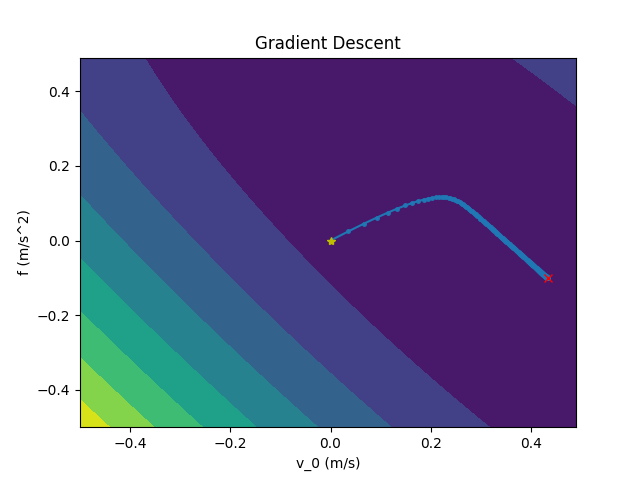
\includegraphics[scale=0.4]{gradient_descent.png}}
\caption{Trajetória de otimização usando Descida do Gradiente.}
\label{gradient_descent}
\end{figure}

\begin{figure}[htbp]
\centering
\centerline{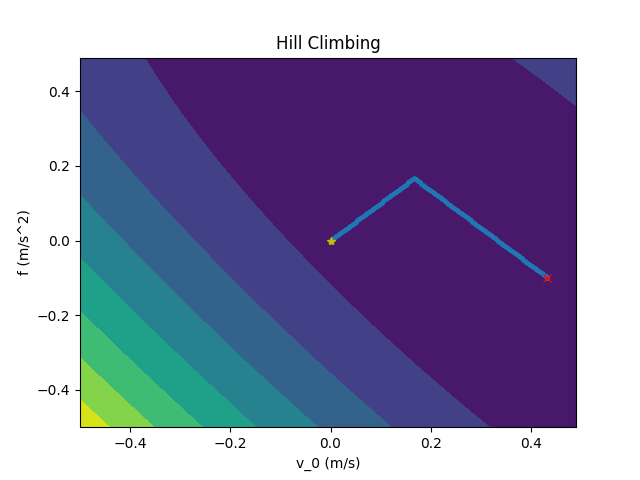
\includegraphics[scale=0.4]{hill_climbing.png}}
\caption{Trajetória de otimização usando Hill Climbing.}
\label{hill_climbing}
\end{figure} 

\begin{figure}[htbp]
\centering
\centerline{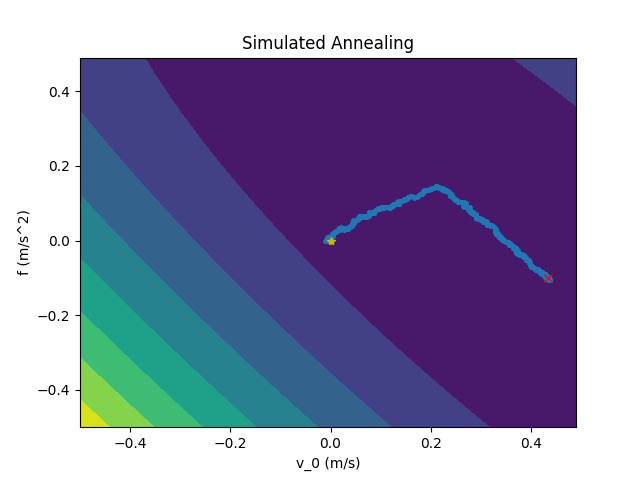
\includegraphics[scale=0.4]{simulated_annealing.png}}
\caption{Trajetória de otimização usando Simulated Annealing.}
\label{simulated_annealing}
\end{figure}

\begin{figure}[htbp]
\centering
\centerline{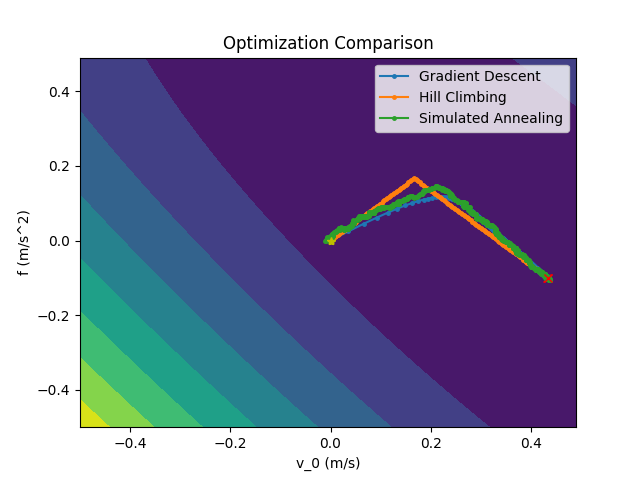
\includegraphics[scale=0.4]{optimization_comparison.png}}
\caption{Comparação de trajetórias de otimização usando Descida do Gradiente, Hill Climbing e Simulated Annealing.}
\label{optimization_comparison}
\end{figure}

Aplicando os valores encontrados para os parâmetros $v_0$ e $f$, o gráfico de velocidade da bola por tempo foi apresentado na Figura \ref{fit_comparison}. Esses valores numéricos de $v_0$ e $f$ podem ser vistos na Tabela \ref{tabelaX} para cada método estudado nesse laboratório, além do resultado fornecido inicialmente para o método de Mínimos Quadrados.

\begin{figure}[H]
\centering
\centerline{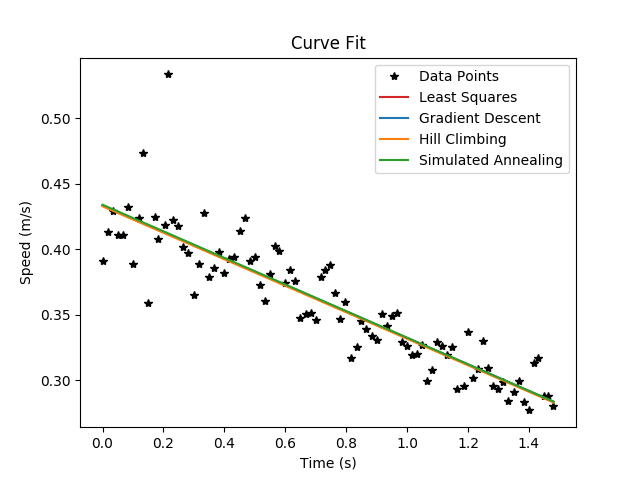
\includegraphics[scale=0.4]{fit_comparison.png}}
\caption{Comparação das regressões lineares das otimizações usando Descida do Gradiente, Hill Climbing e Simulated Annealing.}
\label{fit_comparison}
\end{figure}

\begin{table}[H]
\centering
\caption{Comparação das soluções encontradas para os parâmetros físicos da bola para os algoritmos implementados no laboratório.}
\label{tabelaX}
\begin{tabular}{cc|c|c|c|c|l}
\cline{1-3}
\multicolumn{1}{ |c  }{\multirow{2}{*}{\textbf{Algoritmo}}} & 
\multicolumn{2}{ |c| }{\textbf{Solução}}
\\ \cline{2-3}
\multicolumn{1}{ |c  }{} & 
\multicolumn{1}{ |c  }{\textbf{$v_0$}} & 
\multicolumn{1}{ |c| }{\textbf{$f$}}
\\ \cline{1-3} 
\multicolumn{1}{ |c  }{Mínimos Quadrados} &
\multicolumn{1}{ |c  }{0.43337277} &
\multicolumn{1}{ |c| }{-0.10102096}
\\ \cline{1-3}
\multicolumn{1}{ |c  }{Descida do Gradiente} &
\multicolumn{1}{ |c  }{0.4333707} &
\multicolumn{1}{ |c| }{-0.10101849}
\\ \cline{1-3}
\multicolumn{1}{ |c  }{Hill Climbing} &
\multicolumn{1}{ |c  }{0.43274935} &
\multicolumn{1}{ |c| }{-0.10099495}
\\ \cline{1-3}
\multicolumn{1}{ |c  }{Simulated Annealing} &
\multicolumn{1}{ |c  }{0.43397656} &
\multicolumn{1}{ |c| }{-0.10134529}
\\ \cline{1-3}

\end{tabular}
\end{table}

Tendo em vista o que foi apresentado, pode-se notar, por fim, que esses algoritmos realmente se demonstraram eficazes em encontrar parâmetros otimizados para uma determinada função de custo e um ponto inicial de partida.

\begin{thebibliography}{00}
\bibitem{b1} M. Maximo, ``Roteiro: Laboratório 3 - Otimização com Métodos de Busca Local''. Instituto Tecnológico de Aeronáutica, Departamento de Computação. CT-213, 2019.
\end{thebibliography}

\end{document}
